% !TEX root = main.tex

\section{Introduction}
\label{sec:Introduction}

The weak phase $\gamma$ is the least well known angle of the CKM unitary triangle. 
A key channel to measure $\gamma$ is the time-dependent analysis of $\Bs\to\Ds\kaon$ decays \cite{Fleischer:2003yb}, \cite{DeBruyn:2012jp}. \newline
The $\Bs\to\Ds\kaon\pion\pion$ proceeds at tree level via the transitions shown in Fig. \ref{fig: BsFeynman} a) and b). 

\begin{figure}[h]
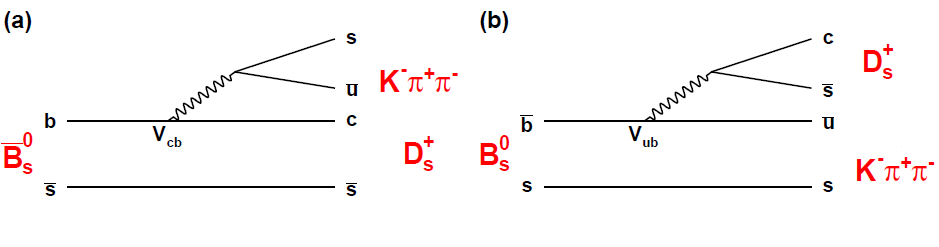
\includegraphics[height=6.cm,width=0.90\textwidth]{figs/FeynmannGraphs.png}
\caption{Feynman diagram of the $\Bs\to\Ds\kaon\pion\pion$ decay, proceeding via a) $\bquark\to\cquark$ transitions or b) $\bquark\to\uquark$ transitions.}
\label{fig: BsFeynman}
\end{figure}

To measure the weak CKM phase $\gamma \equiv arg[-(V_{ud}V_{ub}^{*})/(V_{cd}V_{cb}^{*})]$, a decay with interference between $\bquark\to\cquark$ and $\bquark\to\uquark$ transitions at tree level is needed \cite{Fleischer:2003yb}.
As illustrated in Fig. \ref{fig: BsFeynman}, this is the case for the presented decay mode.  
A measurement of $\gamma$ using $\Bs\to\Ds\kaon\pi\pi$ decays, where the $\kaon\pion\pion$ subsystem 
is dominated by excited kaon states such as the $K_{1}(1270)$ and $K_{1}(1400)$ resonances, will succeed the branching ratio measurement presented in this note.
It is complementary to the above mentioned analysis of $\Bs\to\Ds\kaon$, making use of a fully charged final state, where every track is detected in the vertex locator. 
To account for the non-constant strong phase across the Dalitz plot, 
one can either develop a time-dependent amplitude model 
%bin the phase space and develop a Dalitz model for each bin, 
or select a suitable phase-space region and introduce a coherence factor as additional hadronic parameter to the fit. \newline
This analysis is based on the first observation of the $\Bs\to\Ds\kaon\pion\pion$ decay presented in \cite{Blusk:1471393} and \cite{Blusk:2012it}, where its branching ratio is measured relative to $\Bs\to\Ds\pion\pion\pion$.
The result obtained by the previous analysis is $0.052\mbox{ }\pm 0.005\mbox{ } 0.003$, where the uncertainties are statistical and systematical, respectively.  
The branching ratio measurement is updated, exploiting the full Run 1 data sample, corresponding to 3 $\invfb$ of integrated luminosity.         
